\subsection{Grundlagen}

\subsubsection{Ziel}

TBoxen repräsentieren nur allgemeines, begriffliches Wissen. Um konkrete Situationen zu repräsentieren, braucht man Instanzdaten.

Daher wird in diesem Kapitel ein Formalismus für Instanzdaten (ABox) eingeführt, die Schlussfolgerungsprobleme betrachtet, um mit Instanzdaten zu arbeiten und Anfragebeantwortung mit Datenbanksystemen und Ontologien (Query Rewriting) behandelt.

\subsubsection{ABoxen-Syntax}

\begin{definition}{ABoxen, Syntax}

\begin{itemize}
	\item Eine \emph{Konzerptassertion} hat die Form $A(a)$, $A$ Konzeptname.
	\item Eine Rollenassertion hat die Form $r(a,b)$, $r$ Rollenname.
\end{itemize}

Eine ABox ist eine endlcihe Menge von (Konzept- und Rollen-)assertionen
\end{definition}

\textbf{T7.1}

Eine Beispiel ABox:

\begin{itemize}
	\item $StudentIn(hanna)$
	\item $Person(klaus)$
	\item $bekanntMit(hanna,klaus)$
	\item $TheorieVL(blVl)$
	\item $hoert(hanna, blVl)$
	\item $VL(logikVL)$
\end{itemize}

Mit $Ind(\MA)$ bezeichnen wir die Menge der in $\MA$ verwendeten Individuen.

\subsubsection{ABoxen-Semantik}

\begin{definition}{Aboxen, Semantik}

Interpretation $\MI$

\begin{itemize}
	\item \emph{erfüllt} $A(a)$, wenn $a \in A^{\MI}$;
	\item \emph{erüfllt} $r(a,b)$, wenn $(a,b) \in r^{\MI}$.
\end{itemize}

$\MI$ ist \emph{Modell} von $\MA$, wenn $\MI$ alle Assertionen in $\MA$ erfüllt.
\end{definition}

\textbf{Beachte:}

Modell $\MI$ darf zusätzlich Assertionen wahr machen, die in $\MA$ \emph{nicht} vorkommen.

Das in ABoxen repräsentierte Wissen ist also unvollständiges Wissen.

\textbf{T7.1cont}

Eine Interpretation $\MI$:

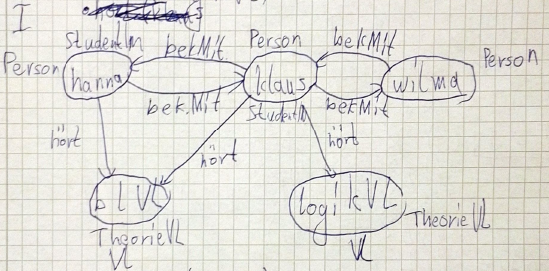
\includegraphics[width=5.21910in,height=2.83200in]{media/71abox.png}

\subsubsection{Wissensbasen}

\begin{definition}

\emph{Wissensbasis (WB)} $\MK = (\MT , \MA)$ besteht aus TBox $\MT$ und ABox $\MA$. Interpretation $\MI$ ist Modell von $\MK$, wenn $\MI$ Modell von $\MT$ und von $\MA$.
\end{definition}

In vielen Anwendungen werden $\MT$ nur einmal erstellt und ändert sich danach üblicherweise nicht mehr, aber $\MA$ ändert sich häufig.

\subsubsection{Grundlegende Schlussfolgerungsprobleme}

\begin{definition}{Konsistenz, Instanz}

Sei $\MK$ Wissensbasis, $A(a)$ Konzeptasertion. Dann ist

\begin{itemize}
	\item $\MK$ \emph{konsistenz}, wenn $\MK$ Modell hat;
	\item $a$ eine Instanz von $A$ bzgl. $\MK$, wenn jedes Modell von $\MK$ auch $A(a)$ erfüllt. Wir schreiben dann $\MK \models A(a)$.
\end{itemize}
\end{definition}

\textbf{T7.2}

$\MK = (\MT, \MA)$

$\MT = \{StudentIn \equiv Person \sqcap \exists hoert.Vl, TheorieVL \sqsubseteq VL\}$

(1) $\MK$ ist konsistent. $\MI$ aus T7.1 erfüllt $(\MT,\MA)$

(2) $\MK' \models StudentIn(klaus)$ mit $\MK' = (\MT, \MA')$ und 

sei $\MA' = \MA \cup \{hoert(klaus,blVL)\}$.

Sei $\MI$ Modell von $\MK'$. 

$\MA'$ liefert $klaus \in Person^{\MI}$, $(klaus,blVL) \in hoert^{\MI}$ und $blVL \in TheorieVL^{\MI}$.

KI2 von $\MT$ liefert $blVL \in VL^{\MI}$

KI1 von $\MT$ liefert $klaus \in StudentIn^{\MI}$

(3) $\MK \not\models TheorieVL(logikVL)$

    ist zwar in $\MI$ aus T7.1 erfüllt, aber setzt man $TheorieVL^{\MI} = \{blVL \}$ so hat man immer noch ein Modell von $\MA,\MT$ 

\textbf{Konsistenzproblem}:

Gegeben $\MK$, entscheide ob $\MK$ konsistent ist.

\textbf{Instanzproblem}:

Gegeben $\MK$ und $A(a)$, entscheide ob $\MK \models A(a)$.

\subsubsection{Reduktionen}

Konsistenz- und (Nicht-)Instanzproblem wechselseitig polynomiell reduzierbar:

\begin{lemma} 

\begin{itemize}
	\item $\MK$ ist konsistent gdw. $\MK \not\models A(a)$, $A$ neuer Konzeptname
	\item $(\MT, \MA) \models A(a)$ gdw. $(\MT \cup \{\MT \cup \{\overline{A} \equiv \neg A\}\})$ inkosistent
\end{itemize}
\end{lemma}

\textbf{T7.3}

(1) $\MK$ konsistenz

gdw. $\MK$ hat Modell

gdw. $\MK$ hat Modell $\MI$ mit $a \not\in A^{\MI}$

gdw. $\MK \not\models A(a)$

(2) $(\MT, \MA) \not\models A(a)$

gdw. es gibt Modell $\MI$ von $(\MT, \MA)$ mit $a \not\in A^{\MI}$ (Def. 7.4)

gdw. es gibt Modell $\MI$ von $(\MT \cup \{\overline{A} \equiv \neg A\}, \MA)$ mit $a \not\in A^{\MI}$

gdw. es gibt Modell $\MI$ von $(\MT \cup \{\overline{A} \equiv \neg A\}, \MA \cup \{\overline{A}(a)\})$

gdw. $(\MT \cup \{\overline{A} \equiv \neg A\}, \MA \cup \{\overline{A}(a)\})$ konsistent

\textbf{T7.2cont}

Instanzanfragen z.B:

StudentIn

Vl

TheorieVl

\textbf{T7.4}

$\MI$ aus Bsp. 7.1

$\Delta^{\MI} = \{hanna, klaus, wilma, blVL, logikVL\}$

$Person^{\MI} = \{hanna,klaus,wilma\}$

$StudentIn^{\MI} = \{hanna,klaus\}$

$TheoVL^{\MI} = VL^{\MI} = \{blVL, logikVL\}$

$bekMit^{\MI} = \{(hanna,klaus), (klaus, hanna), (klaus, wilma), (wilma, klaus)\}$

$hoert^{\MI} = \{(hanna, blVL), (klaus,blVL), (klaus,logikVL)\}$

\begin{tabular}{c | c}
Person & col1 \\ \hline
 & hanna \\
 & klaus \\
 & wilma
\end{tabular}

\begin{tabular}{c | c}
StudentIn & col1 \\ \hline
 & hanna \\
 & klaus
\end{tabular}

\begin{tabular}{c | c | c}
$bekMit^{\MI}$ & col1 & col2 \\ \hline
 & hanna & klaus\\
 & klaus & hanna\\
 & klaus & wilma \\
 & wilma & klaus
\end{tabular}

\textbf{T7.5}

"`Alle StudentInnen, die eine Vorlesung hören"'

$$q_1(\underline{x}) = \exists y (Student(\underline{x}) \wedge hoert(\underline{x},y) \wedge VL(y))$$

"`Alle Paare $(a,b)$ mit $a$ Student, bVL und a hört b"'

$$q_2(\underline{x_1},\underline{x_2}) = Student(\underline{x_1}) \wedge hoert(\underline{x_1},\underline{x_2}) \wedge VL(\underline{x_2})$$

"`Alle Patienten mit Allergien, die ein passendes Medikament bekommen"'

\begin{equation}
\begin{split}
q_3(\underline{x_1}, \underline{x_2}) =& \exists y (Patient(\underline{x_1}) \wedge hat(\underline{x_1},y) \wedge Allergie(y) \wedge erhaelt(\underline{x_1},\underline{x_2}) \\
& \wedge hatAllergen(y,\underline{x_2}) \wedge Medikament(\underline{x_2}))
\end{split}
\end{equation}

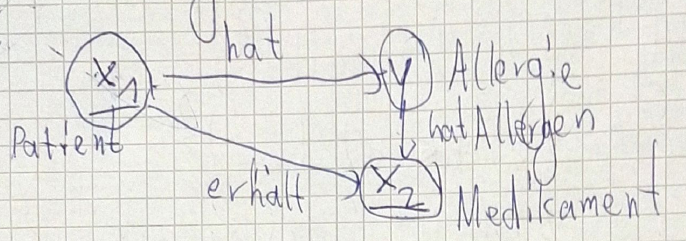
\includegraphics[width=3.81910in,height=1.63200in]{media/75logic.png}

\textbf{T7.6}

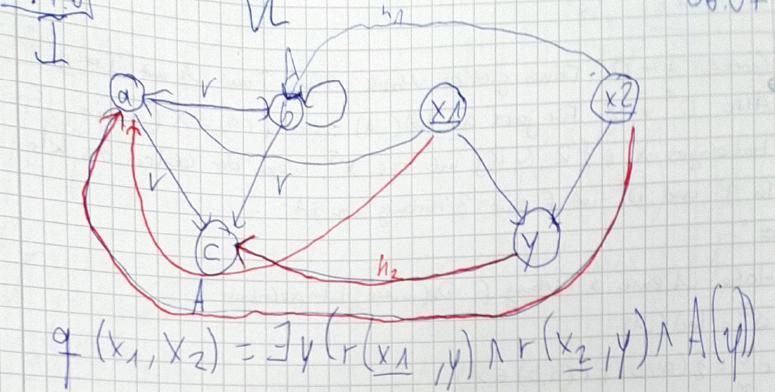
\includegraphics[width=5.81910in,height=3.23200in]{media/76intelog.png}

Homomorph von $q$ auf $\MI$ z.B:

$$x_1 \rightarrow a \quad x_2 \rightarrow b \quad y \rightarrow c$$

$Antwort(a,b)$

oder 

$$x_1 \mapsto a \quad x_2 \mapsto a \quad y \mapsto c$$

Ant(a,a)

und mindestens zwei weitere

\textbf{T7.7}

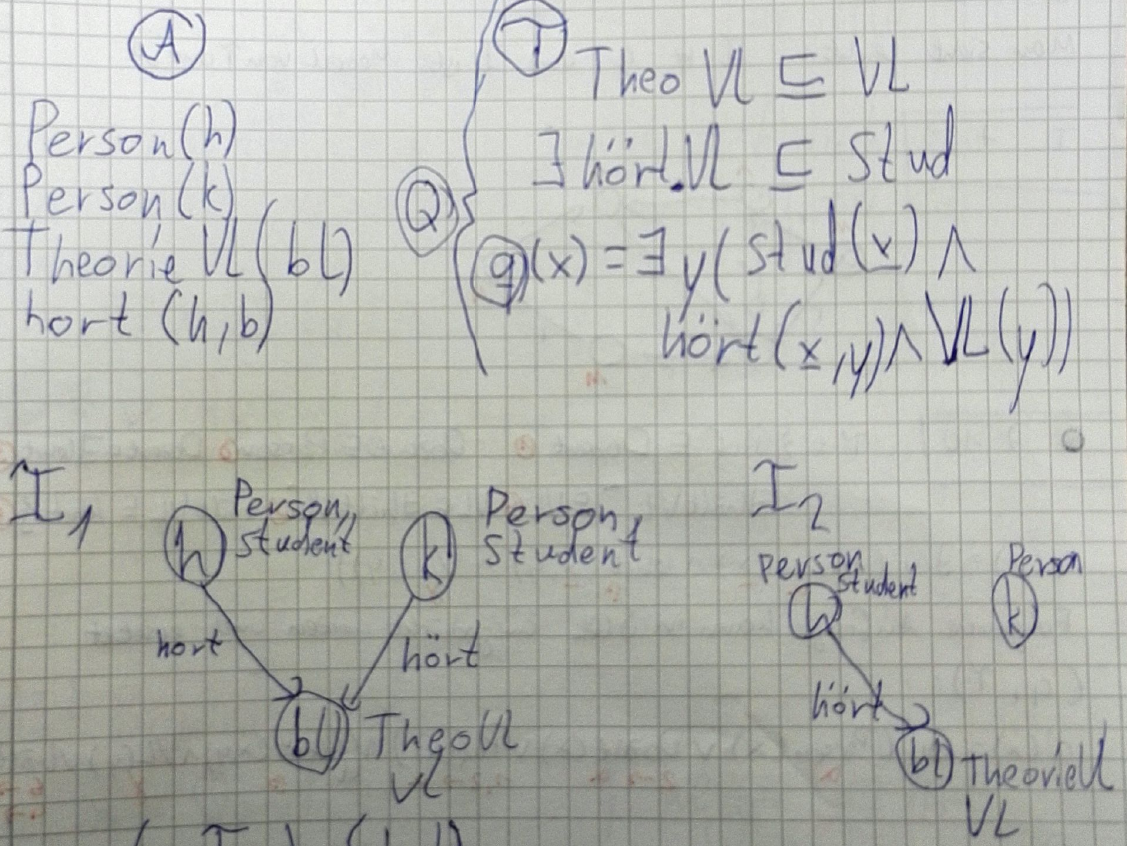
\includegraphics[width=5.81910in,height=5.83200in]{media/77omq.png}

$ans(q, \MI_1) = \{hanna,klaus\}$

$ans(q, \MI_2) = \{hanna\}$

Es gilt: $cert(Q, \MA) = \{h\}$

\textbf{T7.8}

"`$\Leftarrow$"'

Gelte $\MA \not\models Q$. Dann gibt es Modell $\MI$ von $\MT$ und $\MA$ mit $\MI \not\models q$.

Also $D^{\MI} \neq \emptyset$. Für jedes $a \in Ind(\MA)$ setze $f(a) = X$ für ein beliebiges $X \in{R,G,B}$ mit $a \in X^{\MI}$. Wegen der letzten der drei KIs in $\MT$ und $D^{\MI}$ ist $f$ eine 3-Färbung von $\MA$.

"`$\Rightarrow$"'

Habe $\MA$ eine 3-Färbung $f$. Definiere Interpreation $\MI$:

$\Delta^{\MI} = Ind(\MA)$

$r^{\MI} = \{(a,b) | r(a,b) \in \MA \}$

$X^{\MI} = \{a | f(a) = X\}, X \in \{R,G,B\}$

$D^{\MI} = \emptyset$

Man sieht leicht: $\MI \not\models q$ und $\MI$ ist Modell von $\MT$ und $\MA$

\textbf{T7.9}

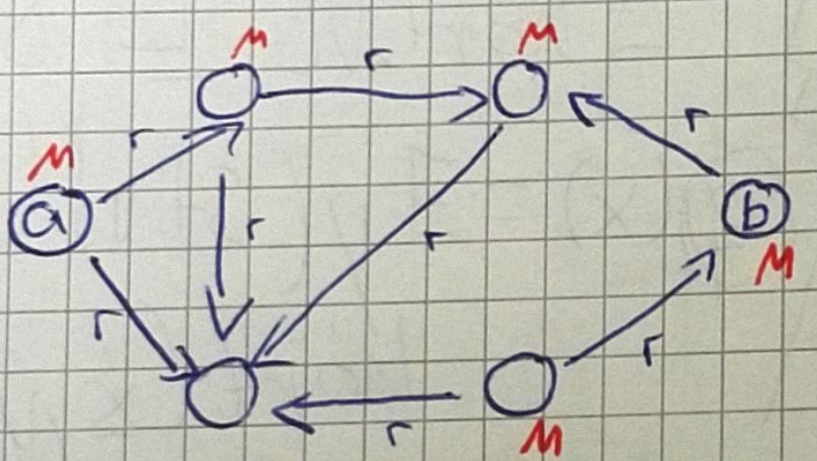
\includegraphics[width=3.81910in,height=1.63200in]{media/79rew.png}

\textbf{T7.10}

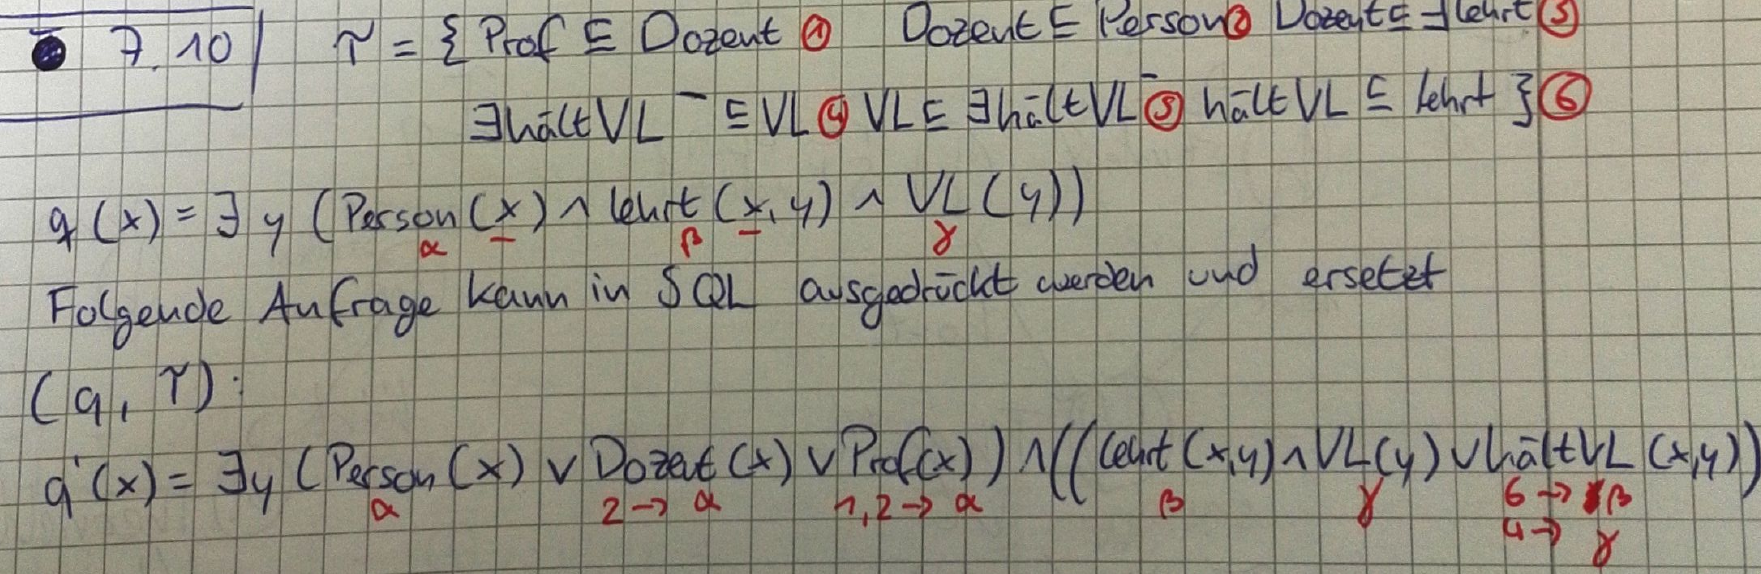
\includegraphics[width=4.81910in,height=2.33200in]{media/710dllite.png}

\textbf{T7.11}

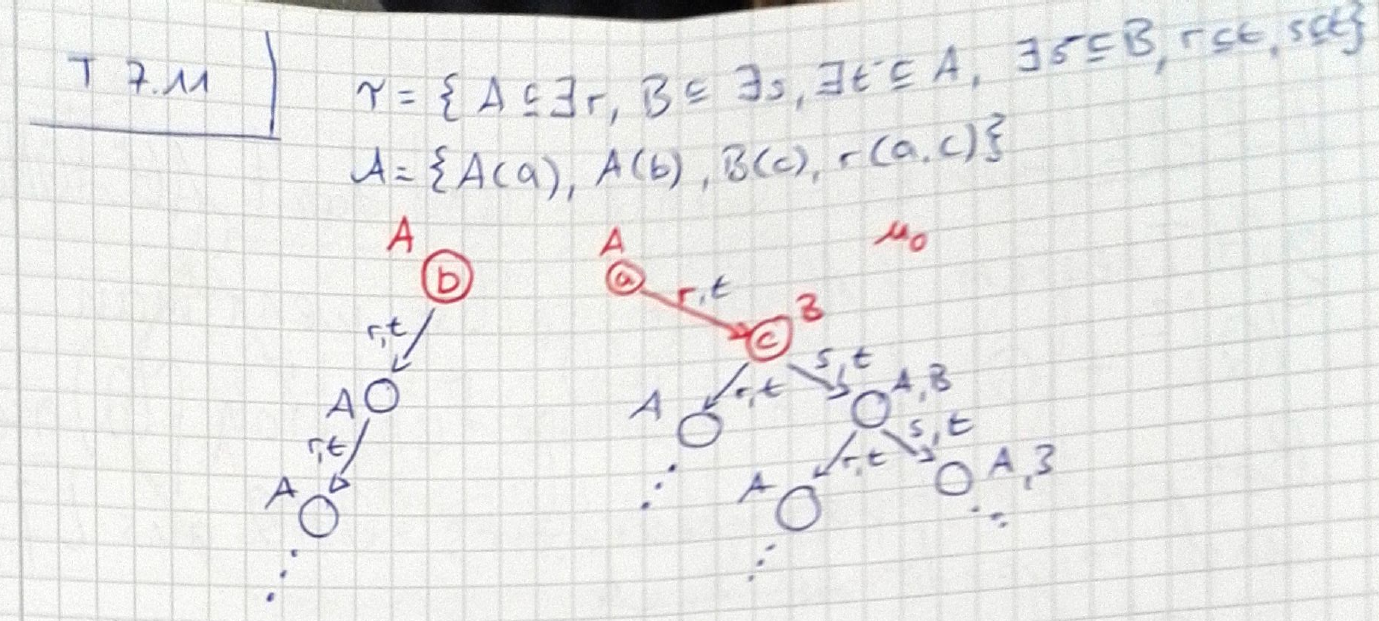
\includegraphics[width=4.81910in,height=2.33200in]{media/711um.png}

\textbf{T7.12}

Für $\EL$-OMQs (und damit $\ALC$-OMQs) gilt Theorem 7.16 nicht, selbst wenn man $|Q|^2 + |Q|$ durch beliebige Funktion $f(Q)$ ersetzt. 

Betrachte Erreichbarkeits-OMQ aus L7.12 und folgende ABox $\MA$

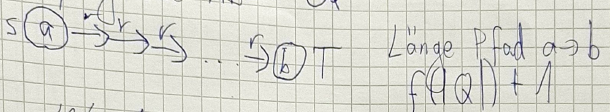
\includegraphics[width=7.41910in,height=1.33200in]{media/712elomq.png}

Es gilt $\MA \models Q$, aber $\MA' \models Q$ für alle $$\MA' \subseteq \MA$$

Nicht Lokalität von Q zeigt sich auch, wenn man naiv versucht, ein Rewriting zu konstruieren:

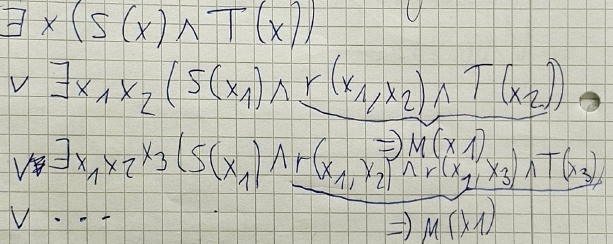
\includegraphics[width=4.41910in,height=2.33200in]{media/712rew.png}

\textbf{T7.13}

Beweisidee

Wenn $\MA = Q$, dann $\MU \models q$ wegen L7.15.

Per Konstruktionen hat $\MU$ folgende Form:

...